\documentclass[12pt,addpoints]{repaso}
\grado{3}
\nivel{Primaria}
\cicloescolar{2025-2026}
\materia{Matemáticas}
\unidad{3}
\title{Practica la Unidad}
\aprendizajes{\scriptsize%
\item Expresa oralmente la sucesión numérica hasta cuatro cifras, en español y hasta donde sea posible, en su lengua materna, de manera ascendente y descendente a partir de un número natural dado.\\[-1.8em]
\item Representa, con apoyo de material concreto y modelos gráficos, fracciones: medios, cuartos, octavos, dieciseisavos, para expresar el resultado de mediciones y repartos en situaciones vinculadas a su contexto.\\[-1.8em]
\item Resuelve situaciones problemáticas vinculadas a su contexto que implican sumas, restas, multiplicación y división de números naturales de hasta tres cifras utilizando el algoritmo convencional y que impliquen, medición, estimación y comparación, de longitudes, masas y capacidades, con el uso del metro, kilogramo, litro y medios y cuartos de estas unidades; en el caso de la longitud, el decímetro y centímetro.\\[-1.8em]
\item Resuelve problemas de suma, resta, multiplicación y división vinculados a su contexto, que impliquen el uso de fracciones (medios, cuartos, octavos, dieciseisavos), con el apoyo de material concreto o representaciones gráficas.
   }
\author{Melchor Pinto, JC}
\begin{document}
\INFO%
% \vfill
\begin{multicols}{1}
	\tableofcontents
\end{multicols}
\newpage
\begin{questions}
	\section{Unidad 1}

	\subsection{Suma de números}

	\questionboxed[6]{Realiza las siguientes sumas:

	\begin{multicols}{4}
		\begin{parts}\large
			\part $9 + 8=$ \fillin[17][0cm]\\[0.2cm]
			\part $5 + 4=$ \fillin[9][0cm]\\[0.2cm]

			\part
			\ifprintanswers{\opadd[hfactor=decimal,resultstyle=\color{red},carryadd=true]{27}{18}}
			\else{\opadd[hfactor=decimal,resultstyle=\color{white},carryadd=false]{27}{18}}\fi\\[0.2cm]

\columnbreak%

			\part $1 + 1=$ \fillin[2][0cm]\\[0.2cm]
			\part $5 + 7=$ \fillin[12][0cm]\\[0.2cm]

			\part
			\ifprintanswers{\opadd[hfactor=decimal,resultstyle=\color{red},carryadd=true]{35}{9}}
			\else{\opadd[hfactor=decimal,resultstyle=\color{white},carryadd=false]{35}{9}}\fi\\[0.2cm]
			
			\columnbreak%
			% \part
			% \ifprintanswers{\opadd[hfactor=decimal,resultstyle=\color{red},carryadd=true]{26}{9}}
			% \else{\opadd[hfactor=decimal,resultstyle=\color{white},carryadd=false]{26}{9}\\[0.5cm]}\fi\\[0.2cm]

			% \part
			% \ifprintanswers{\opadd[hfactor=decimal,resultstyle=\color{red},carryadd=true]{27}{12}}
			% \else{\opadd[hfactor=decimal,resultstyle=\color{white},carryadd=false]{27}{12}}\fi\\[0.2cm]

			\part $0 + 7=$ \fillin[7][0cm]\\[0.2cm]
			\part $8 + 7=$ \fillin[15][0cm]\\[0.2cm]

			\part
			\ifprintanswers{\opadd[hfactor=decimal,resultstyle=\color{red},carryadd=true]{11}{9}}
			\else{\opadd[hfactor=decimal,resultstyle=\color{white},carryadd=false]{11}{9}}\fi\\[0.2cm]
		
			\columnbreak%
			% \part
			% \ifprintanswers{\opadd[hfactor=decimal,resultstyle=\color{red},carryadd=true]{37}{8}}
			% \else{\opadd[hfactor=decimal,resultstyle=\color{white},carryadd=false]{37}{8}\\[0.5cm]}\fi\\[0.2cm]

			% \part
			% \ifprintanswers{\opadd[hfactor=decimal,resultstyle=\color{red},carryadd=true]{48}{14}}
			% \else{\opadd[hfactor=decimal,resultstyle=\color{white},carryadd=false]{48}{14}}\fi\\[0.2cm]

			\part $1 + 9=$ \fillin[10][0cm]\\[0.2cm]
			\part $4 + 9=$ \fillin[13][0cm]\\[0.2cm]

			\part
			\ifprintanswers{\opadd[hfactor=decimal,resultstyle=\color{red},carryadd=true]{31}{19}}
			\else{\opadd[hfactor=decimal,resultstyle=\color{white},carryadd=false]{31}{19}}\fi\\[0.2cm]
			% \part
			% \ifprintanswers{\opadd[hfactor=decimal,resultstyle=\color{red},carryadd=true]{44}{25}}
			% \else{\opadd[hfactor=decimal,resultstyle=\color{white},carryadd=false]{44}{25}\\[0.5cm]}\fi\\[0.2cm]

			% \part
			% \ifprintanswers{\opadd[hfactor=decimal,resultstyle=\color{red},carryadd=true]{82}{38}}
			% \else{\opadd[hfactor=decimal,resultstyle=\color{white},carryadd=false]{82}{38}}\fi\\[0.2cm]
		\end{parts}
	\end{multicols}
}

	\questionboxed[8]{Realiza las siguientes sumas:

		\begin{multicols}{4}
			\begin{parts}
				\part \ifprintanswers{\large  \quad   \opadd[hfactor=decimal,resultstyle=\color{red},carryadd=true,carrysub=false]{38475}{18815} }
				\else{          \large  \quad  \opadd[hfactor=decimal,resultstyle=\color{white},carryadd=false,carrysub=false]{38475}{18815} }
				\fi
				\part \ifprintanswers{\large  \quad   \opadd[hfactor=decimal,resultstyle=\color{red},carryadd=true,carrysub=false]{3234}{24156} }
				\else{          \large  \quad  \opadd[hfactor=decimal,resultstyle=\color{white},carryadd=false,carrysub=false]{3234}{24156} }
				\fi
				% \part \ifprintanswers{\large  \quad   \opadd[hfactor=decimal,resultstyle=\color{red},carryadd=true,carrysub=false]{30985}{19562} }
				% \else{          \large  \quad  \opadd[hfactor=decimal,resultstyle=\color{white},carryadd=false,carrysub=false]{30985}{19562} }
				% \fi
				% \part \ifprintanswers{\large  \quad   \opadd[hfactor=decimal,resultstyle=\color{red},carryadd=true,carrysub=false]{2849}{2415} }
				% \else{          \large  \quad  \opadd[hfactor=decimal,resultstyle=\color{white},carryadd=false,carrysub=false]{2849}{2415} }
				% \fi
				% \part \ifprintanswers{\large  \quad   \opadd[hfactor=decimal,resultstyle=\color{red},carryadd=true,carrysub=false]{31085}{19001} }
				% \else{          \large  \quad  \opadd[hfactor=decimal,resultstyle=\color{white},carryadd=false,carrysub=false]{31085}{19001} }
				% \fi
				% \part \ifprintanswers{\large  \quad   \opadd[hfactor=decimal,resultstyle=\color{red},carryadd=true,carrysub=false]{35701}{25484} }
				% \else{          \large  \quad  \opadd[hfactor=decimal,resultstyle=\color{white},carryadd=false,carrysub=false]{35701}{25484} }
				% \fi
				\part \ifprintanswers{\large  \quad   \opadd[hfactor=decimal,resultstyle=\color{red},carryadd=true,carrysub=false]{46865}{24196} }
				\else{          \large  \quad  \opadd[hfactor=decimal,resultstyle=\color{white},carryadd=false,carrysub=false]{46865}{24196} }
				\fi
				\part \ifprintanswers{\large  \quad   \opadd[hfactor=decimal,resultstyle=\color{red},carryadd=true,carrysub=false]{71858}{5362} }
				\else{          \large  \quad  \opadd[hfactor=decimal,resultstyle=\color{white},carryadd=false,carrysub=false]{71858}{5362} }
				\fi
			\end{parts}
		\end{multicols}
	}

	% \section*{\ifprintanswers{Restas 1                       }
	% \subsection*{Restando con 1, 2 y 3          }
	% \subsection*{Restando con 4, 5, 6, 7, 8 y 9 }
	% \subsection*{Restas como sumas 1            }
	% \subsection*{Restas como suma 2             }
	% \subsection*{Restas como suma 3             }


	% \section*{\ifprintanswers{Restas 2                       }
	% \subsection*{Restas sin transformación 1    }
	% \subsection*{Restas sin transformación 2    }
	% \subsection*{Restas con transformación 1    }
	% \subsection*{Restas con transformación 2    }
	% \subsection*{Restas con transformación 3    }


	\subsection{Resta de números}

\questionboxed[5]{Realiza las siguientes restas:

	\begin{multicols}{4}
		\begin{parts}\large
			\part $9 - 3=$ \fillin[6][0cm]\\[0.2cm]
			% \part $15 - \fillin[8][0.5cm]= 7$\\[0.2cm]

			\part
			\ifprintanswers{\opsub[hfactor=decimal,resultstyle=\color{red},carrysub=true]{17}{6}}
			\else{\opsub[hfactor=decimal,resultstyle=\color{white},carrysub=false]{17}{6}}\fi\\[0.2cm]

			\part
			\ifprintanswers{\opsub[hfactor=decimal,resultstyle=\color{red},carrysub=true]{15}{4}}
			\else{\opsub[hfactor=decimal,resultstyle=\color{white},carrysub=false]{15}{4}}\fi\\[0.2cm]

			% \part
			% \ifprintanswers{\opsub[hfactor=decimal,resultstyle=\color{red},carrysub=true]{34}{22}}
			% \else{\opsub[hfactor=decimal,resultstyle=\color{white},carrysub=false]{34}{22}}\fi\\[0.2cm]

			\part $7 - 4=$ \fillin[3][0cm]\\[0.2cm]
			% \part $12 - \fillin[7][0.5cm]= 5$\\[0.2cm]

			\part
			\ifprintanswers{\opsub[hfactor=decimal,resultstyle=\color{red},carrysub=true]{37}{5}}
			\else{\opsub[hfactor=decimal,resultstyle=\color{white},carrysub=false]{37}{5}}\fi\\[0.2cm]

			\part
			\ifprintanswers{\opsub[hfactor=decimal,resultstyle=\color{red},carrysub=true]{24}{15}}
			\else{\opsub[hfactor=decimal,resultstyle=\color{white},carrysub=false]{24}{15}}\fi\\[0.2cm]

			% \part
			% \ifprintanswers{\opsub[hfactor=decimal,resultstyle=\color{red},carrysub=true]{48}{29}}
			% \else{\opsub[hfactor=decimal,resultstyle=\color{white},carrysub=false]{48}{29}}\fi\\[0.2cm]

			\part $8 - 8=$ \fillin[0][0cm]\\[0.2cm]
			% \part $18 - \fillin[14][0.5cm]= 4$\\[0.2cm]

			\part
			\ifprintanswers{\opsub[hfactor=decimal,resultstyle=\color{red},carrysub=true]{8}{5}}
			\else{\opsub[hfactor=decimal,resultstyle=\color{white},carrysub=false]{8}{5}}\fi\\[0.2cm]

			\part
			\ifprintanswers{\opsub[hfactor=decimal,resultstyle=\color{red},carrysub=true]{16}{9}}
			\else{\opsub[hfactor=decimal,resultstyle=\color{white},carrysub=false]{16}{9}}\fi\\[0.2cm]

			% \part
			% \ifprintanswers{\opsub[hfactor=decimal,resultstyle=\color{red},carrysub=true]{57}{43}}
			% \else{\opsub[hfactor=decimal,resultstyle=\color{white},carrysub=false]{57}{43}}\fi\\[0.2cm]

			\part $11 - 4=$ \fillin[7][0cm]\\[0.2cm]
			% \part $25 - \fillin[20][0.5cm]= 5$\\[0.2cm]

			\part
			\ifprintanswers{\opsub[hfactor=decimal,resultstyle=\color{red},carrysub=true]{14}{5}}
			\else{\opsub[hfactor=decimal,resultstyle=\color{white},carrysub=false]{14}{5}}\fi\\[0.2cm]

			\part
			\ifprintanswers{\opsub[hfactor=decimal,resultstyle=\color{red},carrysub=true]{10}{7}}
			\else{\opsub[hfactor=decimal,resultstyle=\color{white},carrysub=false]{10}{7}}\fi\\[0.2cm]

			% \part
			% \ifprintanswers{\opsub[hfactor=decimal,resultstyle=\color{red},carrysub=true]{63}{18}}
			% \else{\opsub[hfactor=decimal,resultstyle=\color{white},carrysub=false]{63}{18}}\fi\\[0.2cm]
		\end{parts}
	\end{multicols}
}


	\questionboxed[8]{Realiza las siguientes restas:

		\begin{multicols}{4}
			\begin{parts}
				\part \ifprintanswers{\large  \quad   \opsub[hfactor=decimal,resultstyle=\color{red},carryadd=true,carrysub=true]{811}{744} }
				\else{          \large  \quad  \opsub[hfactor=decimal,resultstyle=\color{white},carryadd=false,carrysub=false]{811}{744} }
				\fi
				\part \ifprintanswers{\large  \quad   \opsub[hfactor=decimal,resultstyle=\color{red},carryadd=true,carrysub=true]{4090}{2867} }
				\else{          \large  \quad  \opsub[hfactor=decimal,resultstyle=\color{white},carryadd=false,carrysub=false]{4090}{2867} }
				\fi
				% \part \ifprintanswers{\large  \quad   \opsub[hfactor=decimal,resultstyle=\color{red},carryadd=true,carrysub=true]{3500}{308} }
				% \else{          \large  \quad  \opsub[hfactor=decimal,resultstyle=\color{white},carryadd=false,carrysub=false]{3500}{308} }
				% \fi
				% \part \ifprintanswers{\large  \quad   \opsub[hfactor=decimal,resultstyle=\color{red},carryadd=true,carrysub=true]{3000}{189} }
				% \else{          \large  \quad  \opsub[hfactor=decimal,resultstyle=\color{white},carryadd=false,carrysub=false]{3000}{189} }
				% \fi
				% \part \ifprintanswers{\large  \quad   \opsub[hfactor=decimal,resultstyle=\color{red},carryadd=true,carrysub=true]{1200}{966} }
				% \else{          \large  \quad  \opsub[hfactor=decimal,resultstyle=\color{white},carryadd=false,carrysub=false]{1200}{966} }
				% \fi
				% \part \ifprintanswers{\large  \quad   \opsub[hfactor=decimal,resultstyle=\color{red},carryadd=true,carrysub=true]{3300}{2117} }
				% \else{          \large  \quad  \opsub[hfactor=decimal,resultstyle=\color{white},carryadd=false,carrysub=false]{3300}{2117} }
				% \fi
				% \part \ifprintanswers{\large  \quad   \opsub[hfactor=decimal,resultstyle=\color{red},carryadd=true,carrysub=true]{2000}{1251} }
				% \else{          \large  \quad  \opsub[hfactor=decimal,resultstyle=\color{white},carryadd=false,carrysub=false]{2000}{1251} }
				% \fi
				% \part \ifprintanswers{\large  \quad   \opsub[hfactor=decimal,resultstyle=\color{red},carryadd=true,carrysub=true]{2400}{2023} }
				% \else{          \large  \quad  \opsub[hfactor=decimal,resultstyle=\color{white},carryadd=false,carrysub=false]{2400}{2023} }
				% \fi
				% \part \ifprintanswers{\large  \quad   \opsub[hfactor=decimal,resultstyle=\color{red},carryadd=true,carrysub=false]{2400}{211} }
				% \else{          \large  \quad  \opsub[hfactor=decimal,resultstyle=\color{white},carryadd=false,carrysub=false]{2400}{211} }
				% \fi
				% \part \ifprintanswers{\large  \quad   \opsub[hfactor=decimal,resultstyle=\color{red},carryadd=true,carrysub=false]{1500}{1044} }
				% \else{          \large  \quad  \opsub[hfactor=decimal,resultstyle=\color{white},carryadd=false,carrysub=false]{1500}{1044} }
				% \fi
				\part \ifprintanswers{\large  \quad   \opsub[hfactor=decimal,resultstyle=\color{red},carryadd=true,carrysub=false]{2000}{1105} }
				\else{          \large  \quad  \opsub[hfactor=decimal,resultstyle=\color{white},carryadd=false,carrysub=false]{2000}{1105} }
				\fi
				\part \ifprintanswers{\large  \quad   \opsub[hfactor=decimal,resultstyle=\color{red},carryadd=true,carrysub=false]{1900}{669} }
				\else{          \large  \quad  \opsub[hfactor=decimal,resultstyle=\color{white},carryadd=false,carrysub=false]{1900}{669} }
				\fi
			\end{parts}
		\end{multicols}
	}
		% UNIDAD 2

	% \section*{\ifprintanswers{Tablas de multiplicar 2        }\else{}\fi}
	% \subsection*{\ifprintanswers{Tabla del 6                    }\else{}\fi}
	% \subsection*{\ifprintanswers{Tabla del 7                    }\else{}\fi}
	% \subsection*{\ifprintanswers{Tabla del 8                    }\else{}\fi}
	% \subsection*{\ifprintanswers{Tabla del 9                    }\else{}\fi}
	% \subsection*{\ifprintanswers{Tabla del 10                   }\else{}\fi}
\section{Unidad 2}

	\subsection{Tablas de multiplicar}
	\questionboxed[15]{Reponde las siguientes tablas de multiplicar:

		\begin{multicols}{4}
			\begin{parts}\Large
				\part $7 \times 6=$ \fillin[$42$][0cm]
				\part $9 \times 7=$ \fillin[$63$][0cm]
				\part $6 \times 8=$ \fillin[$48$][0cm]
				\part $6 \times 9=$ \fillin[$54$][0cm]
				\part $4 \times 4=$ \fillin[$16$][0cm]
				\part $7 \times 7=$ \fillin[$49$][0cm]
				\part $7 \times 5=$ \fillin[$35$][0cm]
				\part $5 \times 4=$ \fillin[$20$][0cm]
				\part $8 \times 7=$ \fillin[$56$][0cm]
				\part $3 \times 6=$ \fillin[$18$][0cm]
				\part $5 \times 9=$ \fillin[$45$][0cm]
				\part $5 \times 6=$ \fillin[$30$][0cm]
				\part $3 \times 8=$ \fillin[$24$][0cm]
				\part $2 \times 9=$ \fillin[$18$][0cm]
				\part $2 \times 7=$ \fillin[$14$][0cm]
				\part $4 \times 7=$ \fillin[$28$][0cm]
				\part $3 \times 9=$ \fillin[$27$][0cm]
				\part $5 \times 8=$ \fillin[$40$][0cm]
				\part $6 \times 6=$ \fillin[$36$][0cm]
				\part $7 \times 8=$ \fillin[$56$][0cm]
				\part $9 \times 4=$ \fillin[$36$][0cm]
				\part $8 \times 8=$ \fillin[$64$][0cm]
				\part $9 \times 9=$ \fillin[$81$][0cm]
				\part $6 \times 7=$ \fillin[$42$][0cm]
			\end{parts}
		\end{multicols}
	}

	\questionboxed[15]{Completa las siguientes tablas de multiplicar:

		\begin{multicols}{4}
			\begin{parts}\Large
				\part $\fillin[9][0.5cm] \times 9= 81$
				\part $4 \times \fillin[9][0.5cm]= 36$
				\part $\fillin[7][0.5cm] \times 4= 28$
				\part $\fillin[9][0.5cm] \times 3= 27$
				\part $8 \times \fillin[5][0.5cm]= 40$
				\part $\fillin[6][0.5cm] \times 4= 24$
				\part $7 \times \fillin[7][0.5cm]= 49$
				\part $\fillin[8][0.5cm] \times 3= 24$
				\part $9 \times \fillin[8][0.5cm]= 72$
				\part $10 \times \fillin[10][0.5cm]=100$
				\part $5 \times \fillin[7][0.5cm]=35$
				\part $6 \times \fillin[7][0.5cm]= 42$	
				\part $\fillin[1][0.5cm] \times 9= 9$
				\part $\fillin[6][0.5cm] \times 5= 30$
				\part $\fillin[7][0.5cm] \times 3= 21$
				
				\part $9 \times \fillin[10][0.5cm]=90$

				\part $\fillin[7][0.5cm] \times 8= 56$
				\part $5 \times \fillin[10][0.5cm]=50$
				\part $4 \times \fillin[6][0.5cm]=24$
				\part $1 \times \fillin[7][0.5cm]= 7$	
				\part $\fillin[9][0.5cm] \times 5= 45$
				\part $\fillin[6][0.5cm] \times 6= 36$
				\part $\fillin[8][0.5cm] \times 8= 64$
				\part $\fillin[6][0.5cm] \times 9= 54$
				\part	$3 \times \fillin[10][0.5cm]=30$
				\part $4 \times \fillin[8][0.5cm]=32$
				\part $6 \times \fillin[0][0.5cm]= 0$				
			\end{parts}
		\end{multicols}
	}
% \section*{\ifprintanswers{Multiplicaciones                           }\else{}\fi}
% \subsection*{\ifprintanswers{Multiplicaciones con una cifra 1           }\else{}\fi}
% \subsection*{\ifprintanswers{Multiplicaciones con una cifra 2           }\else{}\fi}
% \subsection*{\ifprintanswers{Multiplicaciones con una cifra 3           }\else{}\fi}
% \subsection*{\ifprintanswers{Multiplicaciones con una cifra 4           }\else{}\fi}
% \subsection*{\ifprintanswers{Multiplicaciones con dos cifras            }\else{}\fi}

\subsection{Multiplicación de números}
	\questionboxed[6]{Realiza las siguientes multiplicaciones:

		\begin{multicols}{3}
			\begin{parts}
				\part \ifprintanswers{\large  \quad   \opmul[hfactor=decimal,resultstyle=\color{red},displayintermediary=None]{314}{2} }
				\else{          \large  \quad  \opmul[hfactor=decimal,resultstyle=\color{white},displayintermediary=None]{314}{2} }
				\fi
				\part \ifprintanswers{\large  \quad   \opmul[hfactor=decimal,resultstyle=\color{red},displayintermediary=None]{283}{4} }
				\else{          \large  \quad  \opmul[hfactor=decimal,resultstyle=\color{white},displayintermediary=None]{283}{4} }
				\fi
				\part \ifprintanswers{\large  \quad   \opmul[hfactor=decimal,resultstyle=\color{red},displayintermediary=None]{2781}{5} }
				\else{          \large  \quad  \opmul[hfactor=decimal,resultstyle=\color{white},displayintermediary=None]{2781}{5} }
				\fi
				\part \ifprintanswers{\large  \quad   \opmul[hfactor=decimal,resultstyle=\color{red},displayintermediary=None]{4914}{6} }
				\else{          \large  \quad  \opmul[hfactor=decimal,resultstyle=\color{white},displayintermediary=None]{4914}{6} }
				\fi
				\part \ifprintanswers{\large  \quad   \opmul[hfactor=decimal,resultstyle=\color{red},displayintermediary=None]{255}{24} }
				\else{          \large  \quad  \opmul[hfactor=decimal,resultstyle=\color{white},displayintermediary=None]{255}{24} }
				\fi
				\part \ifprintanswers{\large  \quad   \opmul[hfactor=decimal,resultstyle=\color{red},displayintermediary=None]{3533}{29} }
				\else{          \large  \quad  \opmul[hfactor=decimal,resultstyle=\color{white},displayintermediary=None]{3533}{29} }
				\fi
			\end{parts}
		\end{multicols}
	}


	% \section*{\ifprintanswers{Divisiones                                 }\else{}\fi}
	% \subsection*{\ifprintanswers{Divisiones del 1 al 5                      }\else{}\fi}
	% \subsection*{\ifprintanswers{Divisiones del 6 al 10                     }\else{}\fi}
	% \subsection*{\ifprintanswers{Divisiones sin residuos                    }\else{}\fi}
	% \subsection*{\ifprintanswers{Divisiones con residuo 1                   }\else{}\fi}
	% \subsection*{\ifprintanswers{Divisiones con residuo 2                   }\else{}\fi}
	\section{Unidad 3}
	\subsection{División de números}

	\questionboxed[8]{Realiza las siguientes divisiones:

		\begin{multicols}{4}
			\begin{parts}
				\part \ifprintanswers{\large\opidiv{123}{6}} \\[0.5em]
				\else{          \Large  \quad $6 \overline{) \ 123\ }$} \\[2em]
				\fi

				\part \ifprintanswers{\large\opidiv{200}{3}} \\[0.5em]
				\else{          \Large  \quad $3 \overline{) \ 200\ }$} \\[2em]
				\fi

				\part \ifprintanswers{\large\opidiv{399}{8}} \\[0.5em]
				\else{          \Large  \quad $8 \overline{) \ 399\ }$} \\[2em]
				\fi

				\part \ifprintanswers{\large\opidiv{193}{7}} \\[0.5em]
				\else{          \Large  \quad $7 \overline{) \ 193\ }$} \\[2em]
				\fi

				\part \ifprintanswers{\large\opidiv{283}{6}} \\[0.5em]
				\else{          \Large  \quad $6 \overline{) \ 283\ }$} \\[2em]
				\fi

				\part \ifprintanswers{\large\opidiv{432}{9}} \\[0.5em]
				\else{          \Large  \quad $9 \overline{) \ 432\ }$} \\[2em]
				\fi

				\part \ifprintanswers{\large\opidiv{644}{8}} \\[0.5em]
				\else{          \Large  \quad $8 \overline{) \ 644\ }$} \\[2em]
				\fi

				\part \ifprintanswers{\large\opidiv{656}{7}} \\[0.5em]
				\else{          \Large  \quad $7 \overline{) \ 656\ }$} \\[2em]
				\fi
			\end{parts}
		\end{multicols}
	}

	% \section*{\ifprintanswers{Introducción a las fracciones              }\else{}\fi}
	% \subsection*{\ifprintanswers{Clasificación de fracciones                }\else{}\fi}

	\subsection{Fracciones}
	\questionboxed[5]{Clasifica las siguientes fracciones en propias, impropias o mixtas:

		\begin{multicols}{5}
			\begin{parts}
				\part $\dfrac{5}{6}$   \fillin[Propia][1cm]   \\[1em]
				\part $5\dfrac{5}{11}$ \fillin[Mixta][1cm]    \\[1em]
				\part $\dfrac{7}{3}$   \fillin[Impropia][1cm] \\[1em]
				\part $\dfrac{3}{4}$   \fillin[Propia][1cm]   \\[1em]
				\part $1\dfrac{2}{3}$  \fillin[Mixta][1cm]    \\[1em]
				\part $\dfrac{7}{5}$   \fillin[Impropia][1cm] \\[1em]
				\part $\dfrac{7}{8}$   \fillin[Propia][1cm]   \\[1em]
				\part $3\dfrac{2}{9}$  \fillin[Mixta][1cm]    \\[1em]
				\part $\dfrac{3}{2}$   \fillin[Impropia][1cm] \\[1em]
				\part $4\dfrac{1}{4}$ \fillin[Mixta][1cm]   \\[1em]
			\end{parts}
		\end{multicols}
	}

	% \subsection*{\ifprintanswers{Representación de fracciones               }\else{}\fi}

	\questionboxed[5]{Escribe sobre la línea la fracción que representa cada imagen:

		\begin{multicols}{5}
			\begin{parts}
				\part 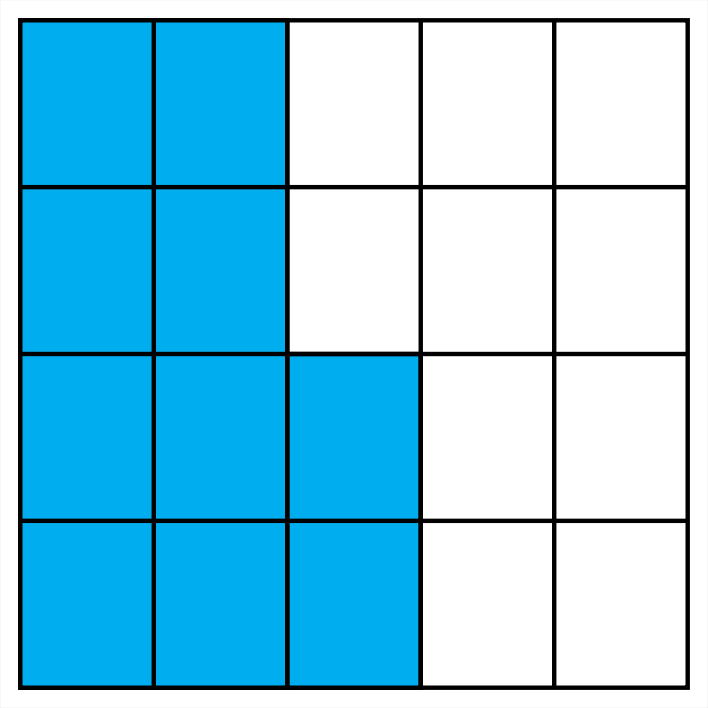
\includegraphics[width=45px]{../images/imagen_frac01.png} \fillin[\fbox{$\dfrac{10}{20}$}][0in] \\[1em]
				\part 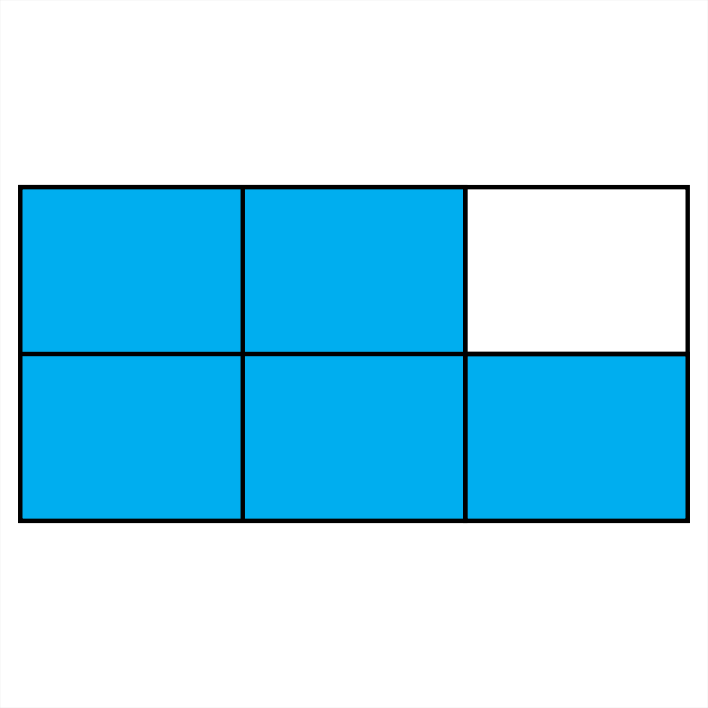
\includegraphics[width=45px]{../images/imagen_frac02.png} \fillin[\fbox{$\dfrac{5}{6}$}][0in] \\[1em]
				\part 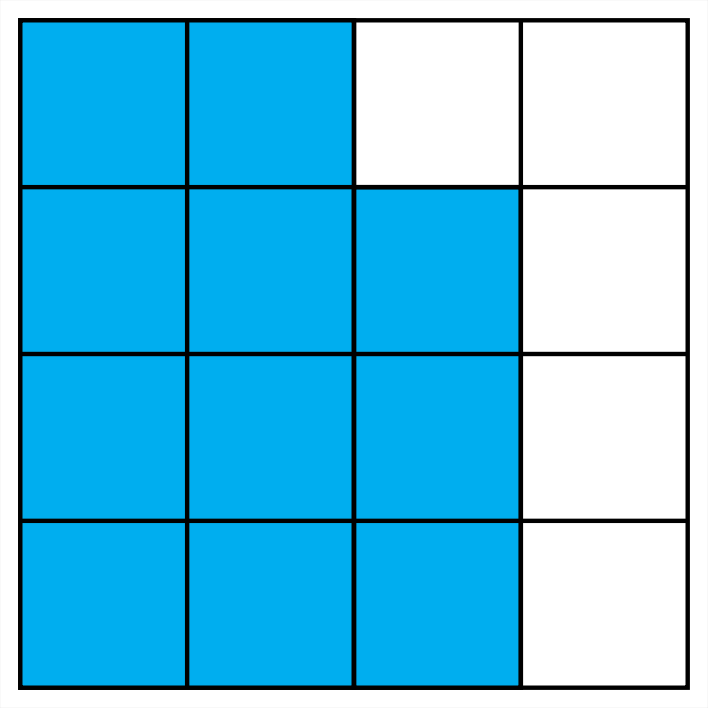
\includegraphics[width=45px]{../images/imagen_frac03.png} \fillin[\fbox{$\dfrac{11}{16}$}][0in] \\[1em]
				\part 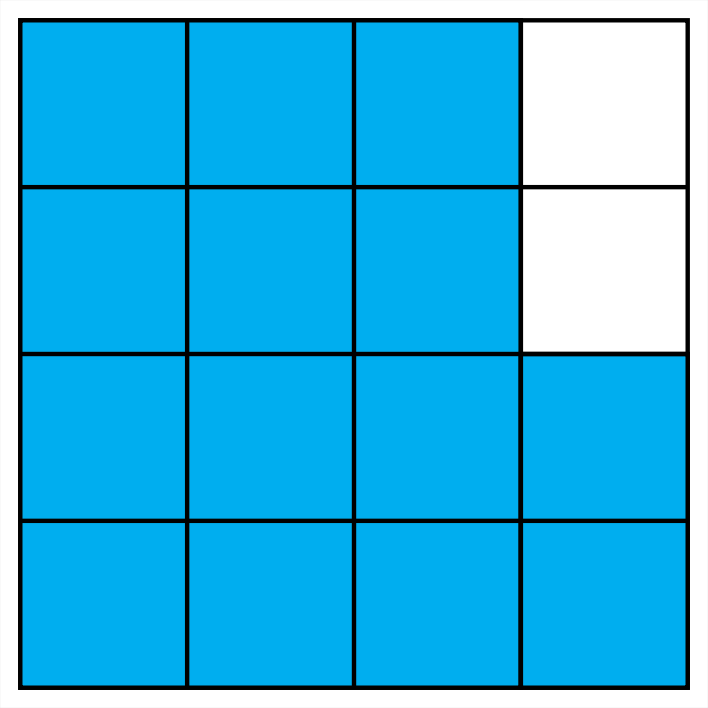
\includegraphics[width=45px]{../images/imagen_frac04.png} \fillin[\fbox{$\dfrac{14}{16}$}][0in] \\[1em]
				\part 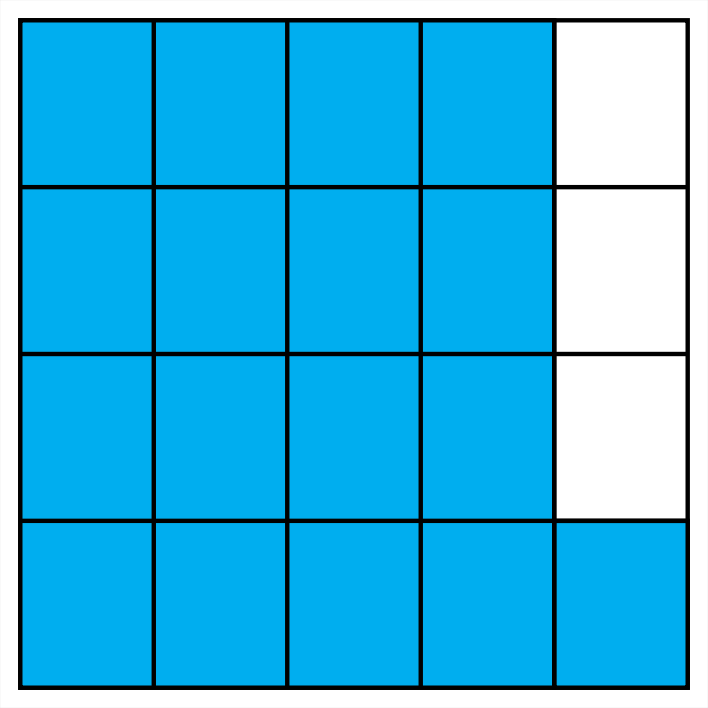
\includegraphics[width=45px]{../images/imagen_frac05.png} \fillin[\fbox{$\dfrac{17}{20}$}][0in] \\[1em]
				\part 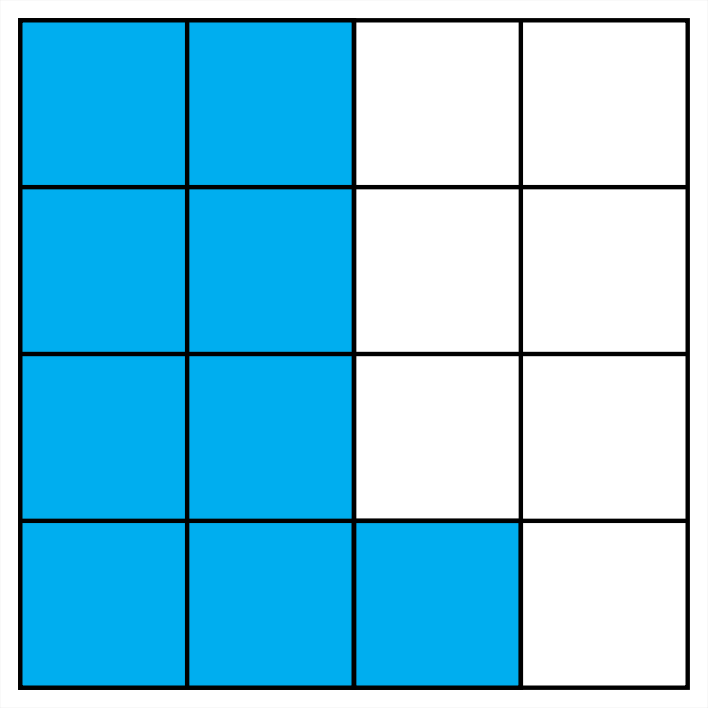
\includegraphics[width=45px]{../images/imagen_frac06.png} \fillin[\fbox{$\dfrac{9}{16}$}][0in] \\[1em]
				\part 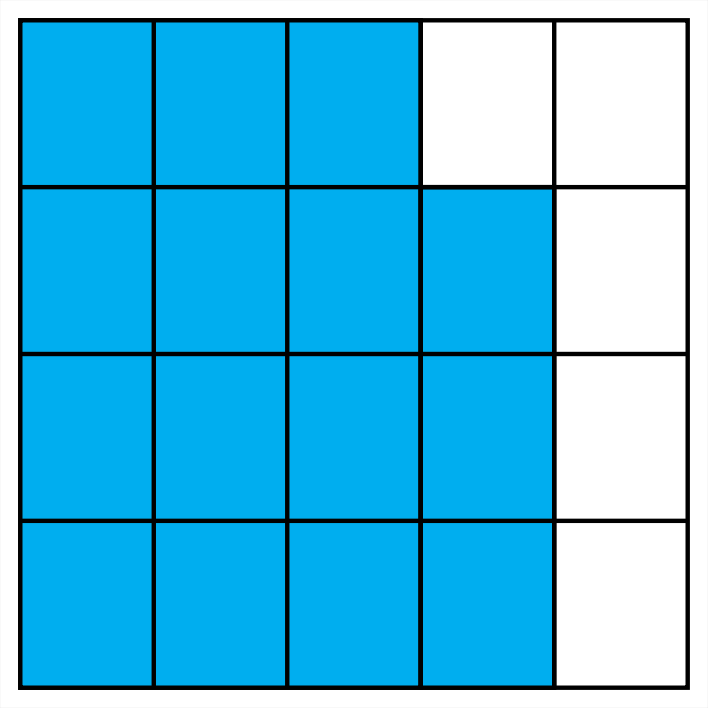
\includegraphics[width=45px]{../images/imagen_frac07.png} \fillin[\fbox{$\dfrac{15}{20}$}][0in] \\[1em]
				\part 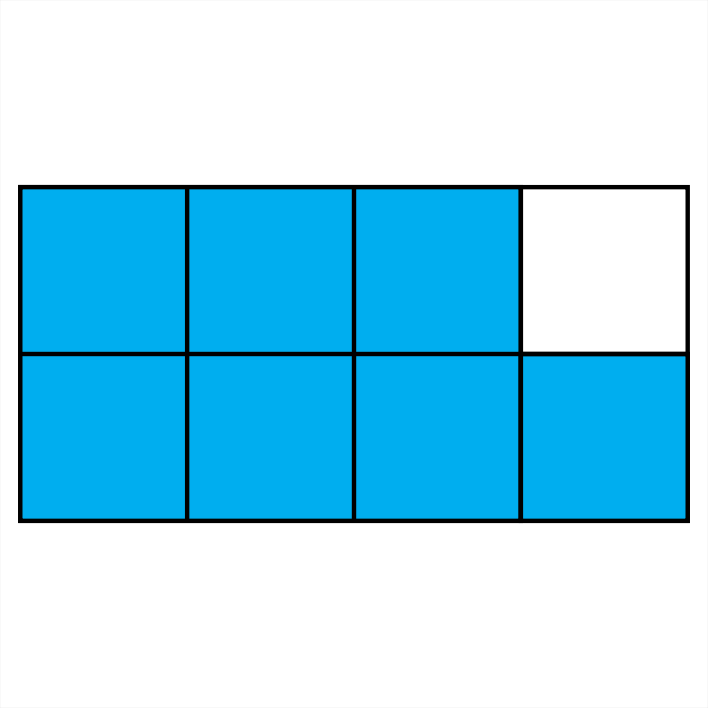
\includegraphics[width=45px]{../images/imagen_frac08.png} \fillin[\fbox{$\dfrac{7}{8}$}][0in] \\[1em]
				\part 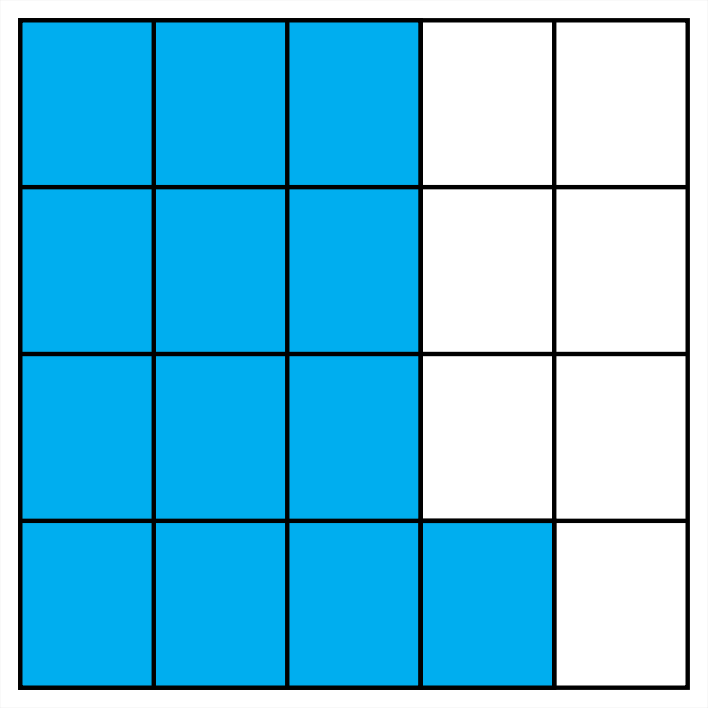
\includegraphics[width=45px]{../images/imagen_frac09.png} \fillin[\fbox{$\dfrac{13}{20}$}][0in] \\[1em]
				\part 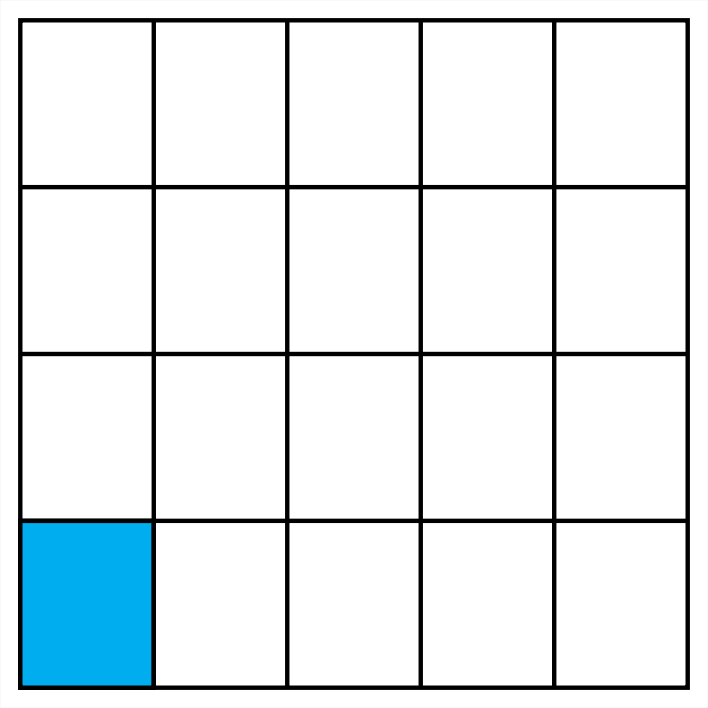
\includegraphics[width=45px]{../images/imagen_frac11.png} \fillin[\fbox{$\dfrac{1}{20}$}][0in] \\[1em]
			\end{parts}
		\end{multicols}
	}


	% \subsection*{\ifprintanswers{Nombre de fracciones                       }\else{}\fi}

	\questionboxed[5]{Escribe la fracción que corresponda en cada inciso:

		\begin{parts}
			\part ¿Cómo se escribe numéricamente la fracción \textbf{ocho quintos}?    \fillin[$\dfrac{8}{5}$][0in]  
			\part ¿Cómo se escribe numéricamente la fracción \textbf{seis onceavos}?   \fillin[$\dfrac{6}{11}$][0in] 
			\part ¿Cómo se escribe numéricamente la fracción \textbf{dos séptimos}?    \fillin[$\dfrac{2}{7}$][0in]  
			\part ¿Cómo se escribe numéricamente la fracción \textbf{once medios}?     \fillin[$\dfrac{11}{2}$][0in] 
			\part ¿Cómo se escribe numéricamente la fracción \textbf{diez décimos}?    \fillin[$\dfrac{10}{10}$][0in]
		\end{parts}
	}

	% \subsection*{\ifprintanswers{Conversión de fracciones mixtas a impropias}\else{}\fi}

	\questionboxed[3]{Convierte la siguientes fracciones mixtas a impropias:

		\begin{multicols}{3}
			\begin{parts}\large
				\part $4\dfrac{2}{3}= $ \fillin[$\dfrac{14}{3}$][0in]
				\part $2\dfrac{3}{10}= $ \fillin[$\dfrac{23}{10}$][0in]
				\part $5\dfrac{1}{5}= $ \fillin[$\dfrac{26}{5}$][0in]
			\end{parts}
		\end{multicols}
	}

	% \subsection*{\ifprintanswers{Conversión de fracciones impropias a mixtas}\else{}\fi}

	\questionboxed[3]{Convierte la siguientes fracciones impropias a mixtas:

		\begin{multicols}{3}
			\begin{parts}\large
				\part $\dfrac{13}{3}= $ \fillin[$4\dfrac{1}{3}$][0in]
				\part $\dfrac{63}{10}= $ \fillin[$6\dfrac{3}{10}$][0in]
				\part $\dfrac{51}{5}= $ \fillin[$10\dfrac{1}{5}$][0in]
			\end{parts}
		\end{multicols}
	}

	% \section*{\ifprintanswers{Operaciones con fracciones                 }\else{}\fi}
	% \subsection*{\ifprintanswers{Suma de fracciones                         }\else{}\fi}
	% \subsection*{\ifprintanswers{Resta de fracciones                        }\else{}\fi}
	% \subsection*{\ifprintanswers{Multiplicación de fracciones               }\else{}\fi}
	% \subsection*{\ifprintanswers{División de fracciones                     }\else{}\fi}
	% \subsection*{\ifprintanswers{Operaciones de fracciones mixtas           }\else{}\fi}

	\subsection{Operaciones con fracciones}

	\questionboxed[8]{Realiza las siguientes operaciones.

		\begin{multicols}{2}
			\begin{parts}\large
				\part $\dfrac{3}{5}+\dfrac{4}{5}=$ \fillin[$\dfrac{7}{5} = 1\dfrac{2}{5}$][0in] \\[2em]
				\part $\dfrac{13}{6}-\dfrac{5}{6}=$ \fillin[$\dfrac{8}{6}=\dfrac{4}{3}$][0in] \\[2em]
				\part $\dfrac{12}{7}-\dfrac{5}{7}=$ \fillin[$\dfrac{7}{7}=1$][0in] \\[2em]
				\part $1\dfrac{1}{8}+1\dfrac{7}{8}=$ \fillin[$2\dfrac{8}{8} = 3$][0in] \\[2em]
				\part $\dfrac{3}{5}\times\dfrac{2}{3}=$ \fillin[$\dfrac{6}{15}$][0in]   \\[2em]
				\part $\dfrac{7}{8}\times\dfrac{3}{4}=$ \fillin[$\dfrac{21}{32}$][0in] \\[2em]
				\part $\dfrac{3}{5} \divisionsymbol\dfrac{2}{3}=$ \fillin[$\dfrac{9}{10}$][0in] \\[2em]
				\part $\dfrac{7}{8} \divisionsymbol\dfrac{3}{4}=$ \fillin[$\dfrac{28}{24}$][0in]	\\[2em]
			\end{parts}
		\end{multicols}
	}
\end{questions}
\end{document}